%%%%%%%%%%%%%%%%%%%%% chapter.tex %%%%%%%%%%%%%%%%%%%%%%%%%%%%%%%%%
%
% sample chapter
%
% Use this file as a template for your own input.
%
%%%%%%%%%%%%%%%%%%%%%%%% Springer-Verlag %%%%%%%%%%%%%%%%%%%%%%%%%%
%\motto{Use the template \emph{chapter.tex} to style the various elements of your chapter content.}
\chapter{Example A: single sector economy}
\chaptermark{Example A}
\label{chap:single_sector} % Always give a unique label
% use \chaptermark{}
% to alter or adjust the chapter heading in the running head

\abstract*{[NEED TO ADD ABSTRACT HERE]}

%% \abstract{Each chapter should be preceded by an abstract (10--15 lines long) that summarizes the content. The abstract will appear \textit{online} at \url{www.SpringerLink.com} and be available with unrestricted access. This allows unregistered users to read the abstract as a teaser for the complete chapter. As a general rule the abstracts will not appear in the printed version of your book unless it is the style of your particular book or that of the series to which your book belongs.\newline\indent
%% Please use the 'starred' version of the new Springer \texttt{abstract} command for typesetting the text of the online abstracts (cf. source file of this chapter template \texttt{abstract}) and include them with the source files of your manuscript. Use the plain \texttt{abstract} command if the abstract is also to appear in the printed version of the book.}

%% Use the template \emph{chapter.tex} together with the Springer document class SVMono (monograph-type books) or SVMult (edited books) to style the various elements of your chapter content in the Springer layout.

In this section, we present an example economic analysis using a single-sector economy wherein the economy and society are merged together.

Figure \ref{fig:single_sector_flows_0} shows a single-sector Economy (represented by ``economy/society,'' 2) that extracts direct energy from the earth ($\dot{E}_{12}$). Direct energy and waste heat flows are identified by vectors. No direct energy flows from the economy (2) to the earth (1), only waste heat ($\dot{Q}_{21}$).

\begin{figure}[h!]
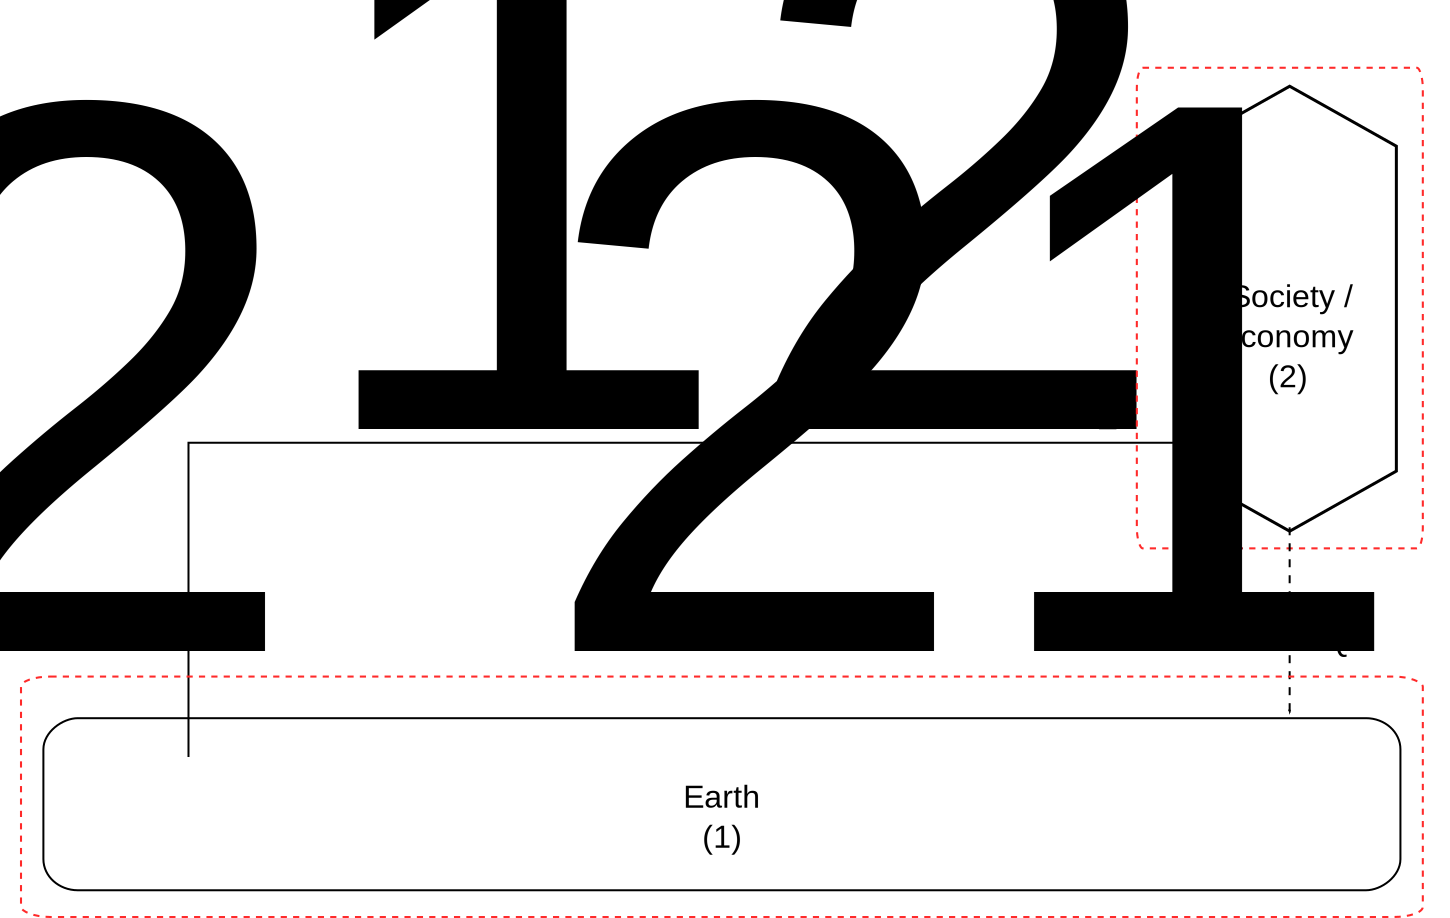
\includegraphics[width=1.0\linewidth]{Chapter_Example_A/images/I-O_one_sector_direct_energy.pdf}
\caption{Direct energy ($\dot{E}$) and waste heat ($\dot{Q}$) flows for a single-sector economy. }
\label{fig:single_sector_flows_0}
\end{figure}

%%%%%%%%%% Example A %%%%%%%%%%
\section{First Law of Thermodynamics}
%%%%%%%%%%

Both direct energy ($\dot{E}$, such as the energy content of coal, oil, and electricity), and waste heat ($\dot{Q}$) are accounted by the First Law of Thermodynamics. Accounting for possible accumulation of direct energy in the economy, the First Law of Thermodynamics indicates that

\begin{equation} \label{eq:dE_2/dt_single_sector}
	\frac{\mathrm{d}E_{2}}{\mathrm{d}t} = \dot{E}_{12} - \dot{Q}_{21}.
\end{equation}

Aside from, for example, the U.S. Strategic Petroleum Reserve, we are not stockpiling oil and coal at any meaningful rate, i.e. we consume fossil fuels at a rate equal to the extraction rate. Thus, the world is not accumulating direct energy in the economy.\footnote{A counter-example could be made for nuclear fuels where `spent' fuel represents a large exergetic stockpile, however, this reserve is not (presently) economically useful.} (The world \emph{is}, however, accumulating embodied energy in the economy as we shall see shortly.) Thus, the accumulation rate for direct energy $\left(\frac{\mathrm{d}E_{2}}{\mathrm{d}t}\right)$ in the above equation can be set to zero to obtain

\begin{equation} \label{eq:single_sector_direct_energy_no_accumulation}
	0 = \dot{E}_{12} - \dot{Q}_{21}.
\end{equation}

%%%%%%%%%% Example A %%%%%%%%%%
\section{Total energy accounting}
%%%%%%%%%%

Figure \ref{fig:single_sector_flows_2} shows the flows of total energy ($\dot{T}$) through the single-sector economy.

\begin{figure}[h!]
\includegraphics[width=1.0\linewidth]{Chapter_Example_A/images/I-O_one_sector_total_energy.pdf}
\caption{Total Energy Flows ($\dot{T}$) in a Single-sector Economy.}
\label{fig:single_sector_flows_2}
\end{figure}

We follow the I-O literature in assuming that total energy ($T$) is conserved. The I-O literature assumes steady-state operation of the economy with no accumulation of embodied energy in the economic sectors. (We will see later how the assumption in the literature introduces errors into I-O analyses.) We depart from the I-O literature by accounting for both accumulation and depreciation of energy embodied in sectors of the economy and society. By doing so, the present analysis does \emph{not} assume a steady-state economy. A total energy accounting around the single-sector economy (2) gives

\begin{equation} \label{eq:single_sector_T_with_accumulation}
	\frac{\mathrm{d}T_{2}}{\mathrm{d}t} = \dot{T}_{12}  - \dot{T}_{21}.
\end{equation}

%%%%%%%%%% Example A %%%%%%%%%%
\section{Embodied energy accounting}
%%%%%%%%%%

The First Law of Thermodynamics accounts for both direct energy ($E$) and waste heat ($Q$), whereas total energy ($T$) accounting tracks direct energy ($E$) and embodied energy ($B$). If we substitute the First Law into the total energy accounting equation, we can eliminate direct energy ($E$) to arrive at an embodied energy accounting equation. We begin by expanding the $T$ terms in Equation \ref{eq:single_sector_T_with_accumulation} using Equations \ref{eq:T_def} and \ref{eq:T_dot_def} to obtain

\begin{equation} \label{eq:single_sector_T_with_accumulation_expanded_T}
	\frac{\mathrm{d}E_{2}}{\mathrm{d}t} + \frac{\mathrm{d}B_{2}}{\mathrm{d}t} = \dot{E}_{12} + \dot{B}_{12} - \dot{E}_{21} - \dot{B}_{21}.
\end{equation}

\noindent Realizing that $\frac{\mathrm{d}E_2}{\mathrm{d}t} = 0$ (because direct energy does not accumulate in meaningful amounts in the economy) and $\dot{E}_{21} = 0$ (because energy is returned to the earth as waste heat, see Figure \ref{fig:single_sector_flows_0}) yields

\begin{equation} \label{eq:single_sector_B_accumulation}
	\frac{\mathrm{d}B_{2}}{\mathrm{d}t} = \dot{E}_{12} + \dot{B}_{12} - \dot{B}_{21}.
\end{equation}

\noindent Equation \ref{eq:single_sector_B_accumulation} shows that the accumulation rate of embodied energy in the economy is a function of the inflows of direct and embodied energy less the outflow of embodied energy. 

In this example, we substitute\footnote{We shall encounter this move to substitute the First Law of Thermodynamics into the total energy accounting equation repeatedly below.} Equation \ref{eq:single_sector_direct_energy_no_accumulation} into Equation \ref{eq:single_sector_B_accumulation} to obtain an embodied energy accounting equation:

\begin{equation} \label{eq:embodied_energy_accounting}
	\frac{\mathrm{d}B_{2}}{\mathrm{d}t} = \dot{Q}_{21} + \dot{B}_{12} - \dot{B}_{21}.
\end{equation}

An important result of Bullard-Herendeen-style I-O analyses, historically, has been the quantification of the embodied energy content of economic sector outputs, in this case $\dot{B}_{21}$. Equation \ref{eq:single_sector_B_accumulation} can be rearranged to give

\begin{equation} \label{eq:single_sector_B_output}
	\dot{B}_{21} = \dot{Q}_{21} + \dot{B}_{12} - \frac{\mathrm{d}B_{2}}{\mathrm{d}t}.
\end{equation}

Equation \ref{eq:single_sector_B_output} indicates that the embodied energy content of the product of an economic sector (in this case $\dot{B}_{21}$) can be thought of as the sum of the embodied energy inputs to the sector (in this case $\dot{B}_{12}$) and the waste heat from the sector (in this case $\dot{Q}_{21}$) less the accumulation rate of embodied energy in the sector (in this case $\frac{\mathrm{d}B_{2}}{\mathrm{d}t}$). This derivation indicates that waste heat ($\dot{Q}$) plays an important role\footnote{To our knowledge, there has been no prior identification of the role of waste heat in Bullard-Herendeen-style I-O analyses.} in Bullard-Herendeen-style I-O analyses: the accumulation of waste heat along a production path leads to energy being `embodied' in the output of an economic sector. 

In Equation \ref{eq:single_sector_B_output} we also see the first indication that the traditional approach of neglecting dynamic effects in I-O analyses may lead to errors. If $\frac{\mathrm{d}B_2}{\mathrm{d}t}$ is both neglected and nonzero, calculation of the embodied energy outflow rate ($\dot{B}_{21}$) will be in error.

%%%%%%%%%% Example A %%%%%%%%%%
\section{Depreciation}
%%%%%%%%%%

It is worthwhile to note that $\dot{B}_{21}$ represents the disposal rate of embodied energy from the economy back to the earth, akin to depreciation of physical assets. This physical depreciation is different from, but related to, financial depreciation, as financial depreciation is usually faster than physical depreciation. Embodied energy depreciation ($\dot{B}_{21}$ in this example) can be represented by a depreciation term such as

\begin{equation} \label{eq:depreciation_term_defined}
	\dot{B}_{21} = \gamma_{2}B_{2},
\end{equation}

\noindent where $\gamma$ represents the depreciation rate in units of inverse time (e.g., 1/year) with $\gamma > 0$. The depreciation rate ($\gamma$) indicates that a fraction of the total stock of embodied energy is disposed over a period of time (e.g, $\gamma = 0.05$/year). In the absence of other inputs or outputs, this depreciation function provides exponential decay of embodied energy ($B$). $\gamma$ is, in general, a function of time.

Equation \ref{eq:depreciation_term_defined} can be substituted into Equation \ref{eq:embodied_energy_accounting} and rearranged to obtain 

\begin{equation} \label{eq:dB2/dt_single_sector_with_depreciation_gamma}
	\frac{\mathrm{d}B_{2}}{\mathrm{d}t} =  \dot{Q}_{21} + \dot{B}_{12} - \gamma_{2}B_{2}
\end{equation}

\noindent which indicates that the accumulation rate of embodied energy in an economic sector (in this case $\frac{\mathrm{d}B_{2}}{\mathrm{d}t}$) is equal to the sum of the waste heat rate from the economic sector ($\dot{Q}_{21}$) and the inflow rate of embodied energy to the sector ($\dot{B}_{12}$) less the embodied energy disposal rate ($\gamma_{2}B_{2}$).


\bibliography{EROI_review_v2}
\bibliographystyle{unsrt}


% Always give a unique label
% and use \ref{<label>} for cross-references
% and \cite{<label>} for bibliographic references
% use \sectionmark{}
% to alter or adjust the section heading in the running head
%% Instead of simply listing headings of different levels we recommend to let every heading be followed by at least a short passage of text. Furtheron please use the \LaTeX\ automatism for all your cross-references and citations.

%% Please note that the first line of text that follows a heading is not indented, whereas the first lines of all subsequent paragraphs are.

%% Use the standard \verb|equation| environment to typeset your equations, e.g.
%
%% \begin{equation}
%% a \times b = c\;,
%% \end{equation}
%
%% however, for multiline equations we recommend to use the \verb|eqnarray|
%% environment\footnote{In physics texts please activate the class option \texttt{vecphys} to depict your vectors in \textbf{\itshape boldface-italic} type - as is customary for a wide range of physical subjects.}.
%% \begin{eqnarray}
%% a \times b = c \nonumber\\
%% \vec{a} \cdot \vec{b}=\vec{c}
%% \label{eq:01}
%% \end{eqnarray}

%% \subsection{Subsection Heading}
%% \label{subsec:2}
%% Instead of simply listing headings of different levels we recommend to let every heading be followed by at least a short passage of text. Furtheron please use the \LaTeX\ automatism for all your cross-references\index{cross-references} and citations\index{citations} as has already been described in Sect.~\ref{sec:2}.

%% \begin{quotation}
%% Please do not use quotation marks when quoting texts! Simply use the \verb|quotation| environment -- it will automatically render Springer's preferred layout.
%% \end{quotation}


%% \subsubsection{Subsubsection Heading}
%% Instead of simply listing headings of different levels we recommend to let every heading be followed by at least a short passage of text. Furtheron please use the \LaTeX\ automatism for all your cross-references and citations as has already been described in Sect.~\ref{subsec:2}, see also Fig.~\ref{fig:1}\footnote{If you copy text passages, figures, or tables from other works, you must obtain \textit{permission} from the copyright holder (usually the original publisher). Please enclose the signed permission with the manucript. The sources\index{permission to print} must be acknowledged either in the captions, as footnotes or in a separate section of the book.}

%% Please note that the first line of text that follows a heading is not indented, whereas the first lines of all subsequent paragraphs are.

% For figures use
%
%% \begin{figure}[b]
%% \sidecaption
% Use the relevant command for your figure-insertion program
% to insert the figure file.
% For example, with the option graphics use
%% \includegraphics[scale=.65]{figure}
%
% If not, use
%\picplace{5cm}{2cm} % Give the correct figure height and width in cm
%
%% \caption{If the width of the figure is less than 7.8 cm use the \texttt{sidecapion} command to flush the caption on the left side of the page. If the figure is positioned at the top of the page, align the sidecaption with the top of the figure -- to achieve this you simply need to use the optional argument \texttt{[t]} with the \texttt{sidecaption} command}
%% \label{fig:1}       % Give a unique label
%% \end{figure}


%% \paragraph{Paragraph Heading} %
%% Instead of simply listing headings of different levels we recommend to let every heading be followed by at least a short passage of text. Furtheron please use the \LaTeX\ automatism for all your cross-references and citations as has already been described in Sect.~\ref{sec:2}.

%% Please note that the first line of text that follows a heading is not indented, whereas the first lines of all subsequent paragraphs are.

%% For typesetting numbered lists we recommend to use the \verb|enumerate| environment -- it will automatically render Springer's preferred layout.

%% \begin{enumerate}
%% \item{Livelihood and survival mobility are oftentimes coutcomes of uneven socioeconomic development.}
%% \begin{enumerate}
%% \item{Livelihood and survival mobility are oftentimes coutcomes of uneven socioeconomic development.}
%% \item{Livelihood and survival mobility are oftentimes coutcomes of uneven socioeconomic development.}
%% \end{enumerate}
%% \item{Livelihood and survival mobility are oftentimes coutcomes of uneven socioeconomic development.}
%% \end{enumerate}


%% \subparagraph{Subparagraph Heading} In order to avoid simply listing headings of different levels we recommend to let every heading be followed by at least a short passage of text. Use the \LaTeX\ automatism for all your cross-references and citations as has already been described in Sect.~\ref{sec:2}, see also Fig.~\ref{fig:2}.

%% Please note that the first line of text that follows a heading is not indented, whereas the first lines of all subsequent paragraphs are.

%% For unnumbered list we recommend to use the \verb|itemize| environment -- it will automatically render Springer's preferred layout.

%% \begin{itemize}
%% \item{Livelihood and survival mobility are oftentimes coutcomes of uneven socioeconomic development, cf. Table~\ref{tab:1}.}
%% \begin{itemize}
%% \item{Livelihood and survival mobility are oftentimes coutcomes of uneven socioeconomic development.}
%% \item{Livelihood and survival mobility are oftentimes coutcomes of uneven socioeconomic development.}
%% \end{itemize}
%% \item{Livelihood and survival mobility are oftentimes coutcomes of uneven socioeconomic development.}
%% \end{itemize}

%% \begin{figure}[t]
%% \sidecaption[t]
% Use the relevant command for your figure-insertion program
% to insert the figure file.
% For example, with the option graphics use
%% \includegraphics[scale=.65]{figure}
%
% If not, use
%\picplace{5cm}{2cm} % Give the correct figure height and width in cm
%
%% \caption{Please write your figure caption here}
%% \label{fig:2}       % Give a unique label
%% \end{figure}

%% \runinhead{Run-in Heading Boldface Version} Use the \LaTeX\ automatism for all your cross-references and citations as has already been described in Sect.~\ref{sec:2}.

%% \subruninhead{Run-in Heading Italic Version} Use the \LaTeX\ automatism for all your cross-refer\-ences and citations as has already been described in Sect.~\ref{sec:2}\index{paragraph}.
% Use the \index{} command to code your index words
%
% For tables use
%
%% \begin{table}
%% \caption{Please write your table caption here}
%% \label{tab:1}       % Give a unique label
%
% For LaTeX tables use
%
%% \begin{tabular}{p{2cm}p{2.4cm}p{2cm}p{4.9cm}}
%% \hline\noalign{\smallskip}
%% Classes & Subclass & Length & Action Mechanism  \\
%% \noalign{\smallskip}\svhline\noalign{\smallskip}
%% Translation & mRNA$^a$  & 22 (19--25) & Translation repression, mRNA cleavage\\
%% Translation & mRNA cleavage & 21 & mRNA cleavage\\
%% Translation & mRNA  & 21--22 & mRNA cleavage\\
%%Translation & mRNA  & 24--26 & Histone and DNA Modification\\
%%\noalign{\smallskip}\hline\noalign{\smallskip}
%%\end{tabular}
%%$^a$ Table foot note (with superscript)
%%\end{table}
%
%% \section{Section Heading}
%%\label{sec:3}
% Always give a unique label
% and use \ref{<label>} for cross-references
% and \cite{<label>} for bibliographic references
% use \sectionmark{}
% to alter or adjust the section heading in the running head
%% Instead of simply listing headings of different levels we recommend to let every heading be followed by at least a short passage of text. Furtheron please use the \LaTeX\ automatism for all your cross-references and citations as has already been described in Sect.~\ref{sec:2}.

%% Please note that the first line of text that follows a heading is not indented, whereas the first lines of all subsequent paragraphs are.

%%If you want to list definitions or the like we recommend to use the Springer-enhanced \verb|description| environment -- it will automatically render Springer's preferred layout.

%%\begin{description}[Type 1]
%%\item[Type 1]{That addresses central themes pertainng to migration, health, and disease. In Sect.~\ref{sec:1}, Wilson discusses the role of human migration in infectious disease distributions and patterns.}
%%\item[Type 2]{That addresses central themes pertainng to migration, health, and disease. In Sect.~\ref{subsec:2}, Wilson discusses the role of human migration in infectious disease distributions and patterns.}
%%\end{description}

%%\subsection{Subsection Heading} %
%% In order to avoid simply listing headings of different levels we recommend to let every heading be followed by at least a short passage of text. Use the \LaTeX\ automatism for all your cross-references and citations citations as has already been described in Sect.~\ref{sec:2}.

%% Please note that the first line of text that follows a heading is not indented, whereas the first lines of all subsequent paragraphs are.

%% \begin{svgraybox}
%% If you want to emphasize complete paragraphs of texts we recommend to use the newly defined Springer class option \verb|graybox| and the newly defined environment \verb|svgraybox|. This will produce a 15 percent screened box 'behind' your text.

%% If you want to emphasize complete paragraphs of texts we recommend to use the newly defined Springer class option and environment \verb|svgraybox|. This will produce a 15 percent screened box 'behind' your text.
%% \end{svgraybox}


%% \subsubsection{Subsubsection Heading}
%%Instead of simply listing headings of different levels we recommend to let every heading be followed by at least a short passage of text. Furtheron please use the \LaTeX\ automatism for all your cross-references and citations as has already been described in Sect.~\ref{sec:2}.

%% Please note that the first line of text that follows a heading is not indented, whereas the first lines of all subsequent paragraphs are.

%% \begin{theorem}
%% Theorem text goes here.
%% \end{theorem}
%
% or
%
%% \begin{definition}
%% Definition text goes here.
%% \end{definition}

%% \begin{proof}
%\smartqed
%% Proof text goes here.
%% \qed
%% \end{proof}

%%\paragraph{Paragraph Heading} %
%% Instead of simply listing headings of different levels we recommend to let every heading be followed by at least a short passage of text. Furtheron please use the \LaTeX\ automatism for all your cross-references and citations as has already been described in Sect.~\ref{sec:2}.

%% Note that the first line of text that follows a heading is not indented, whereas the first lines of all subsequent paragraphs are.
%
% For built-in environments use
%
%%\begin{theorem}
%%Theorem text goes here.
%%\end{theorem}
%
%%\begin{definition}
%%Definition text goes here.
%%\end{definition}
%
%%\begin{proof}
%%\smartqed
%% Proof text goes here.
%%\qed
%%\end{proof}
%
%% \begin{acknowledgement}
%% If you want to include acknowledgments of assistance and the like at the end of an individual chapter please use the \verb|acknowledgement| environment -- it will automatically render Springer's preferred layout.
%% \end{acknowledgement}
%
%% \section*{Appendix}
%% \addcontentsline{toc}{section}{Appendix}
%
%% When placed at the end of a chapter or contribution (as opposed to at the end of the book), the numbering of tables, figures, and equations in the appendix section continues on from that in the main text. Hence please \textit{do not} use the \verb|appendix| command when writing an appendix at the end of your chapter or contribution. If there is only one the appendix is designated ``Appendix'', or ``Appendix 1'', or ``Appendix 2'', etc. if there is more than one.

%% \begin{equation}
%% a \times b = c
%% \end{equation}
% Problems or Exercises should be sorted chapterwise
%% \section*{Problems}
%% \addcontentsline{toc}{section}{Problems}
%
% Use the following environment.
% Don't forget to label each problem;
% the label is needed for the solutions' environment
%% \begin{prob}
%% \label{prob1}
%% A given problem or Excercise is described here. The
%% problem is described here. The problem is described here.
%% \end{prob}

%% \begin{prob}
%% \label{prob2}
%% \textbf{Problem Heading}\\
%% (a) The first part of the problem is described here.\\
%% (b) The second part of the problem is described here.
%% \end{prob}


